% Options for packages loaded elsewhere
\PassOptionsToPackage{unicode}{hyperref}
\PassOptionsToPackage{hyphens}{url}
%
\documentclass[
]{article}
\usepackage{lmodern}
\usepackage{amssymb,amsmath}
\usepackage{ifxetex,ifluatex}
\ifnum 0\ifxetex 1\fi\ifluatex 1\fi=0 % if pdftex
  \usepackage[T1]{fontenc}
  \usepackage[utf8]{inputenc}
  \usepackage{textcomp} % provide euro and other symbols
\else % if luatex or xetex
  \usepackage{unicode-math}
  \defaultfontfeatures{Scale=MatchLowercase}
  \defaultfontfeatures[\rmfamily]{Ligatures=TeX,Scale=1}
\fi
% Use upquote if available, for straight quotes in verbatim environments
\IfFileExists{upquote.sty}{\usepackage{upquote}}{}
\IfFileExists{microtype.sty}{% use microtype if available
  \usepackage[]{microtype}
  \UseMicrotypeSet[protrusion]{basicmath} % disable protrusion for tt fonts
}{}
\makeatletter
\@ifundefined{KOMAClassName}{% if non-KOMA class
  \IfFileExists{parskip.sty}{%
    \usepackage{parskip}
  }{% else
    \setlength{\parindent}{0pt}
    \setlength{\parskip}{6pt plus 2pt minus 1pt}}
}{% if KOMA class
  \KOMAoptions{parskip=half}}
\makeatother
\usepackage{xcolor}
\IfFileExists{xurl.sty}{\usepackage{xurl}}{} % add URL line breaks if available
\IfFileExists{bookmark.sty}{\usepackage{bookmark}}{\usepackage{hyperref}}
\hypersetup{
  hidelinks,
  pdfcreator={LaTeX via pandoc}}
\urlstyle{same} % disable monospaced font for URLs
\usepackage[margin=1in]{geometry}
\usepackage{longtable,booktabs}
% Correct order of tables after \paragraph or \subparagraph
\usepackage{etoolbox}
\makeatletter
\patchcmd\longtable{\par}{\if@noskipsec\mbox{}\fi\par}{}{}
\makeatother
% Allow footnotes in longtable head/foot
\IfFileExists{footnotehyper.sty}{\usepackage{footnotehyper}}{\usepackage{footnote}}
\makesavenoteenv{longtable}
\usepackage{graphicx,grffile}
\makeatletter
\def\maxwidth{\ifdim\Gin@nat@width>\linewidth\linewidth\else\Gin@nat@width\fi}
\def\maxheight{\ifdim\Gin@nat@height>\textheight\textheight\else\Gin@nat@height\fi}
\makeatother
% Scale images if necessary, so that they will not overflow the page
% margins by default, and it is still possible to overwrite the defaults
% using explicit options in \includegraphics[width, height, ...]{}
\setkeys{Gin}{width=\maxwidth,height=\maxheight,keepaspectratio}
% Set default figure placement to htbp
\makeatletter
\def\fps@figure{htbp}
\makeatother
\setlength{\emergencystretch}{3em} % prevent overfull lines
\providecommand{\tightlist}{%
  \setlength{\itemsep}{0pt}\setlength{\parskip}{0pt}}
\setcounter{secnumdepth}{-\maxdimen} % remove section numbering

\author{}
\date{\vspace{-2.5em}}

\begin{document}

\hypertarget{case-study-1-interior-fraser-coho-salmon}{%
\section{CASE STUDY 1: INTERIOR FRASER COHO
SALMON}\label{case-study-1-interior-fraser-coho-salmon}}

\hypertarget{context}{%
\subsection{CONTEXT}\label{context}}

The Interior Fraser Coho Salmon Stock Management Unit (SMU) includes
Coho Salmon that return to the Fraser River and tributaries upstream of
Hell's Gate in the Fraser Canyon. Like most coho salmon, IF Coho spend
at least one full year in freshwater as fry before migrating to the
ocean as smolts {[}@arbeider\_interior\_2020{]}. Most (88\%) IFC have a
3-year life cycle, in which they leave freshwater in their second year
and spend 18 months at sea prior to returning to their natal system to
spawn. The remaining 12\% have a 4-year life cycle in which they spend
an additional year in freshwater before migrating as smolts in their
third year. Both 3-year and 4-year life cycles spend 18 months at sea.
Less than 1\% of IF Coho are believed to return as jacks (precocious
mature males that spend only 6 months as sea) or at ages older than 4
years {[}@arbeider\_interior\_2020{]}.

WSP Conservation Units (CUs) have been identified for of Interior Fraser
Coho based on genetics and geographic separation: Middle Fraser, Fraser
Canyon, Lower Thompson, North Thompson, and South Thompson
{[}@dfo\_wild\_2015; Figure @ref(fig:coho-map){]}. Previous work by the
Interior Fraser Coho Recovery Team identified 11 subpopulations nested
within the five CUs, and developed recovery objectives based on
maintaining abundance in each of these smaller subpopulation units
{[}@ifcrt\_interior\_fraser\_coho\_recovery\_team\_conservation\_2006;
Table @ref(tab:cohoCU2SP){]}. The delineation of subpopulations was
based on several factors, including the presence of natural barriers,
the influence of large lakes on downstream discharge and thermal
regimes, observations of spawner aggregations under differing discharge
conditions, and genetic evidence. The 11 subpopulations are described in
detail by the
@ifcrt\_interior\_fraser\_coho\_recovery\_team\_conservation\_2006. The
Fraser Canyon CU is the only CU with a single subpopulation; this result
is because most of the spawning for the CU occurs within a single river
{[}@arbeider\_interior\_2020{]}.

\begin{figure}

{\centering 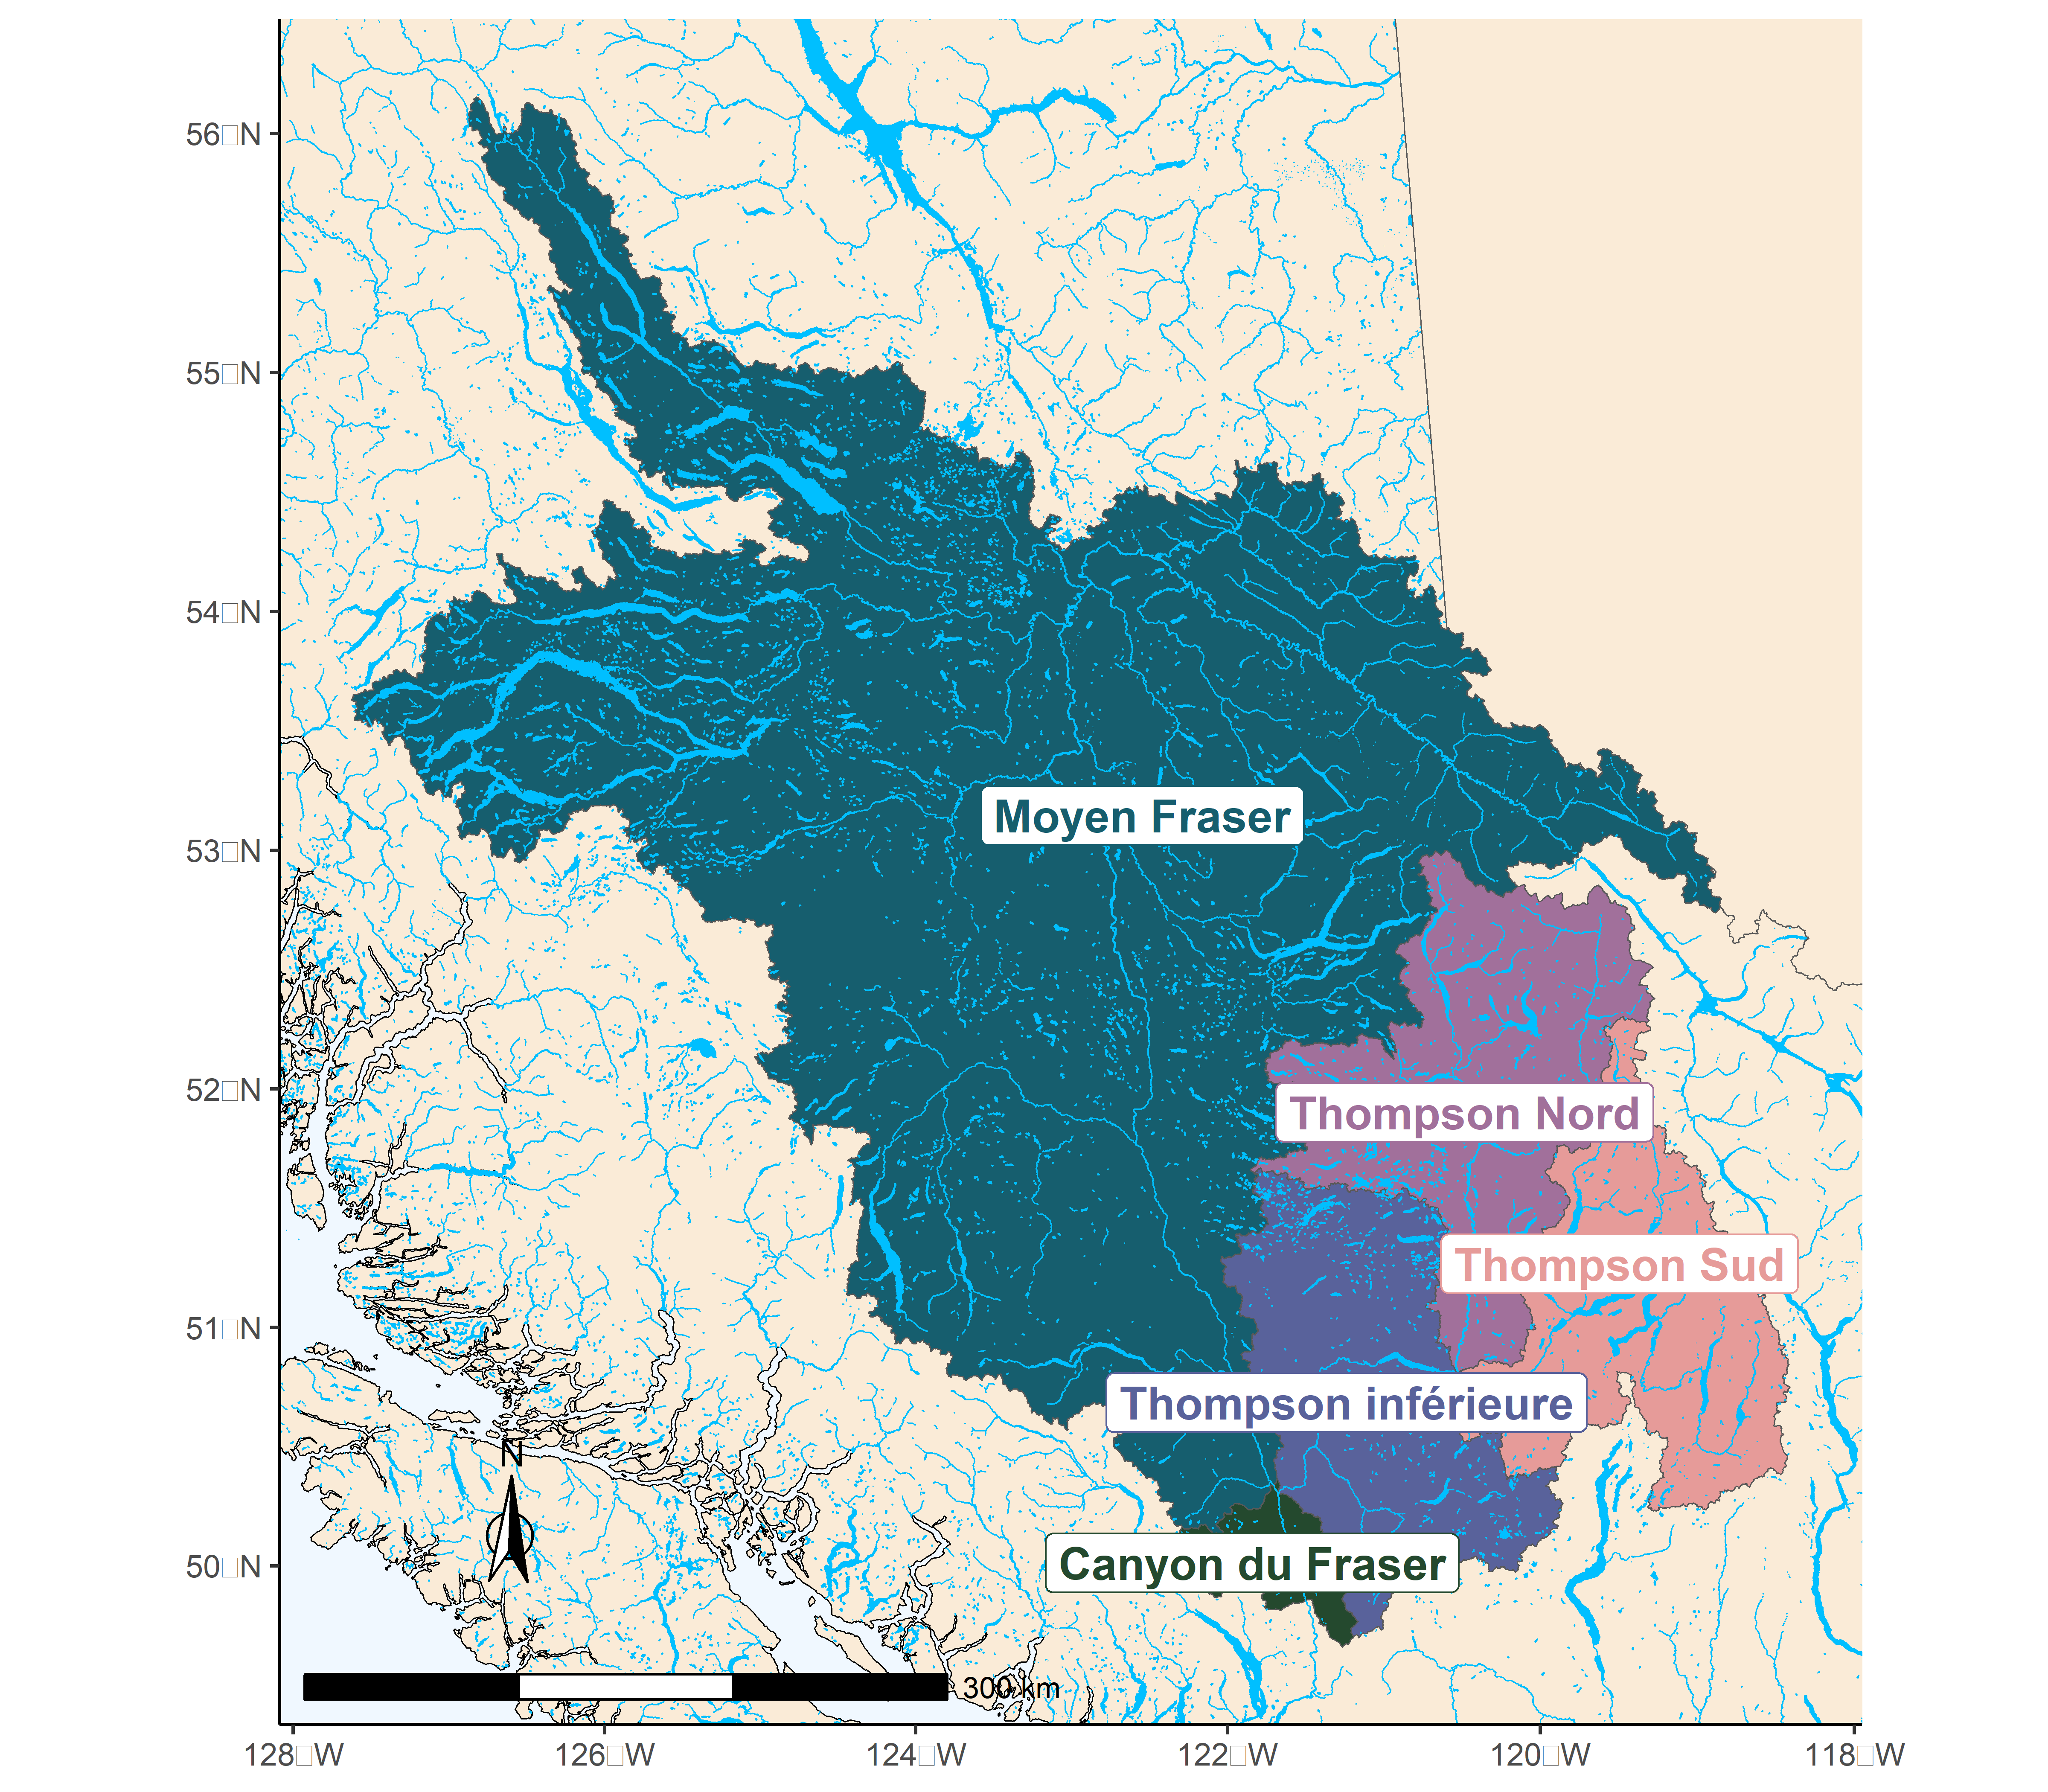
\includegraphics[width=0.6\linewidth]{figure/coho-map} 

}

\caption{The five Conservation Units that make up the Interior Fraser Coho Stock Management Unit.}\label{fig:coho-map}
\end{figure}

\begin{longtable}[]{@{}ll@{}}
\caption{(\#tab:cohoCU2SP) Interior Fraser Coho Conservation Units (CUs)
and associated sub-populations. Note that the definition of these
sub-populations, including mapped boundaries, are provided in
@ifcrt\_interior\_fraser\_coho\_recovery\_team\_conservation\_2006.}\tabularnewline
\toprule
\begin{minipage}[b]{0.26\columnwidth}\raggedright
Conservation Unit\strut
\end{minipage} & \begin{minipage}[b]{0.43\columnwidth}\raggedright
Sub-populations\strut
\end{minipage}\tabularnewline
\midrule
\endfirsthead
\toprule
\begin{minipage}[b]{0.26\columnwidth}\raggedright
Conservation Unit\strut
\end{minipage} & \begin{minipage}[b]{0.43\columnwidth}\raggedright
Sub-populations\strut
\end{minipage}\tabularnewline
\midrule
\endhead
\begin{minipage}[t]{0.26\columnwidth}\raggedright
Middle Fraser\strut
\end{minipage} & \begin{minipage}[t]{0.43\columnwidth}\raggedright
\begin{itemize}
\tightlist
\item
  Lower Middle Fraser
\item
  Upper Middle Fraser
\end{itemize}\strut
\end{minipage}\tabularnewline
\begin{minipage}[t]{0.26\columnwidth}\raggedright
Fraser Canyon\strut
\end{minipage} & \begin{minipage}[t]{0.43\columnwidth}\raggedright
\begin{itemize}
\tightlist
\item
  Nahatlatch
\end{itemize}\strut
\end{minipage}\tabularnewline
\begin{minipage}[t]{0.26\columnwidth}\raggedright
Lower Thompson\strut
\end{minipage} & \begin{minipage}[t]{0.43\columnwidth}\raggedright
\begin{itemize}
\tightlist
\item
  Lower Thompson
\item
  Nicola
\end{itemize}\strut
\end{minipage}\tabularnewline
\begin{minipage}[t]{0.26\columnwidth}\raggedright
North Thompson\strut
\end{minipage} & \begin{minipage}[t]{0.43\columnwidth}\raggedright
\begin{itemize}
\tightlist
\item
  Lower North Thompson
\item
  Middle Thompson
\item
  Upper North Thompson
\end{itemize}\strut
\end{minipage}\tabularnewline
\begin{minipage}[t]{0.26\columnwidth}\raggedright
South Thompson\strut
\end{minipage} & \begin{minipage}[t]{0.43\columnwidth}\raggedright
\begin{itemize}
\tightlist
\item
  Adams Drainage
\item
  Lower and Middle Shuswap Rivers
\item
  Shuswap Lake Tributaries
\end{itemize}\strut
\end{minipage}\tabularnewline
\bottomrule
\end{longtable}

Declines in IF Coho spawner abundance throughout the 1990's led to a
suite of management actions to promote recovery, including significant
fishery restrictions starting in 1998 {[}@decker\_assessment\_2014{]}.
Evidence of a new, lower productivity regime starting in return year
1994 has been documented {[}@decker\_assessment\_2014{]} that coincides
with declines in spawner abundances. In 2002, the IF Coho stock
management unit was designated `endangered; by the Committee on the
Status of Endangered Wildlife in Canada (COSWEIC) based on the stock
unit being assessed as a single 'Designatable Unit' (DU). Subsequent
work by the Interior Fraser Coho Recovery Team (IFCRT) lead to a
conservation strategy outlining recovery objectives for the management
unit
(@ifcrt\_interior\_fraser\_coho\_recovery\_team\_conservation\_2006).
Those recovery objectives were largely based on the distribution of
spawning escapement among 11 subpopulations(Table @ref(tab:cohoCU2SP)).
The delineation of subpopulations was based on several factors,
including the presence of natural barriers, the influence of large lakes
on downstream discharge and thermal regimes, observations of spawner
aggregations under differing discharge conditions, and genetic evidence.
The 11 subpopulations are described in detail by the
@ifcrt\_interior\_fraser\_coho\_recovery\_team\_conservation\_2006. The
IFCRT identified a short-term recovery objective of 20,000 spawners,
which represented the level that was expected to maintain a minimum of
1,000 naturally spawning wild Coho Salmon in at least half of the 11
subpopulations. In addition, the IFCRT identified a long-term recovery
target of 40,000 spawners, which represented a level that was expected
to maintain 1,000 or more wild Coho Salmon in all 11 subpopulations. In
2014, @decker\_assessment\_2014 assessed status relative to the 2006
IFCRT objectives, and concluded that IF coho had been above the
short-term recovery target of 20,000 spawners in every year since 2008,
and above the long-term recovery target of 40,000 spawners in the most
recent two return years (2012 and 2013)

In 2014, Interior Fraser Coho were assessed under the framework of DFO's
Wild Salmon Policy (WSP), at which time the Integrated Status Assessment
classified three of these CUs as being amber status (Middle Fraser,
Fraser Canyon, South Thompson) and the remaining two CUs as amber/green
status (Lower Thompson, North Thompson; {[}@dfo\_wild\_2015{]}). A
subsequent COSEWIC assessment in 2016 upgraded the status designation
for the IF Coho DU from `endangered' to `threatened'
{[}@cosewic\_cosewic\_2016{]}. In 2018, DFO undertook a Recovery
Potential Assessment (RPA) for Interior Fraser Coho that described
status, habitat, threats, limiting factors to recovery, candidate
recovery targets, and abundance projections for the DU, as well as
recommendations regarding mitigation and allowable harm
{[}@arbeider\_interior\_2020{]}. As part of this RPA, the long-term DU
recovery target for IF Coho was recommended was a 3-year geometric mean
abundance of 35,935 natural-origin spawners. This target was based on
the historically observed aggregate abundance that met the long-term
IFCRT objective of 1000 spawners in all subpopulations.

To Do: need to work in @korman\_evaluation\_2019

\hypertarget{data}{%
\subsection{DATA}\label{data}}

Data for this case study cover return years 1998 -2020. Data prior to
1998 were not used due to concerns about inconsistent assessment methods
and data quality. All Interior Fraser Coho data were provided by DFO's
Fraser River Stock Assessment Unit (M. Arbeider, pers. comm). These data
included: (i) annual spawner abundance by CU (1998-2020), (ii) annual
recruits-at-age by CU (brood years 1998 - 2016), (iii) a hatchery-based
smolt-to-adult survival rate index, (iv) annual exploitation rates, and
(v) annual spawner abundances for 11 sub-populations nested within the 5
CUs. Data were similar to those previously described in
@arbeider\_interior\_2020; data treatments, assumptions, infilling, and
data quality are described in detail in that document. More recent
updates that are not described in @arbeider\_interior\_2020 include the
incorporation of three additional years of data (return years
2018-2020), updates to the smolt-to-adult marine survival rate index to
use a weighted average by release size, and increased data quality
screening of scale ages used to calculate recruitment-at-age (M.
Arbeider, pers. comm).

\begin{itemize}
\tightlist
\item
  Still to add:
\item
  Highlight high among-CU correlation
\item
  Caveats: e.g., recruitment estimated using common ER for all CUs;
  review Arbeider et al.~for additional data caveats
\end{itemize}

\hypertarget{methods}{%
\subsection{METHODS}\label{methods}}

\hypertarget{cu-status-estimation}{%
\subsubsection{CU Status Estimation}\label{cu-status-estimation}}

We consider two types of CU benchmark to represent CU status when
developing LRPs for Interior Fraser Coho.

\textbf{Sgen}

The first type is the WSP lower benchmark of \(S_{gen}\), where Sgen is
the number of spawners required to recover to SMSY (spawners maximum
sustainable yield) within one generation, under equilibrium conditions
in the absence of fishing {[}@holt\_indicators\_2009{]}. Four different
formulations of stock recruitment model are used to estimate Sgen based
on previous analyses. Key differences among the formulations centre
around whether a hierarchical model structure is used when estimating
Sgen and whether an informative prior distribution is applied to the
spawner abundance level at which the stock replaced itself (SRep).

We primarily use the two model formulations that assume no hierarchical
structure among CUs (IM and IM.cap) as a basis for comparing among LRP
estimation methods, but have retained the two hierarchical model
formulations (HM and HM.cap) for sensitivity analyses. Our rationale for
focusing on the individual modelling approaches was two-fold. First,
because all CUs had equal amounts of data, the commonly cited benefit of
hierarchical models allowing data-poor systems to borrow information
from data-rich systems did not apply. Second, initial investigations of
the hierarchical models fit to IF coho data showed that LRP estimates
were sensitive to the choice of the assumed standard deviation on the
hyper-distribution for the productivity parameter.

\emph{Model 1: Individual Ricker (IM)}

Using this approach, we assumed that productivity was independent among
CUs with a shared covariate for marine survival. The Individual Ricker
stock recruit model formulation was:

\begin{equation}
  \hat{R}_{i,a,t} = P_{i,a,t-a}S_{i,t-a}e^{log(\alpha_i) + \gamma log(m_{t-1})-\beta_i S_{i,t-a}e^{v_i}}
   (\#eq:rickerSurv-IM)
\end{equation} \begin{equation}
  v_i \sim Normal(0,\sigma_{v_i})
\end{equation}

where,

\(\hat{R}_{i,a,t}\) = the predicted number of natural origin recruits
from CU \(i\) of age \(a\) returning in year \(t\) (i.e., recruits that
were produced by escapement in brood year \(t-a\))

\(P_{i,a,t-a}\) = the proportion of recruitment from CU \(i\) returning
at age \(a\) from brood year \(t-a\)

\(S_{i,t-a}\) = spawners from CU \(i\) in brood year \(t-a\)

\(\alpha_i\) = productivity parameter for CU \(i\)

\(\gamma\) = marine survival co-efficient shared among CUs

\(m_{t-1}\) = hatchery marine survival index (smolt-to-adult) for sea
entry in year t-1

\(\beta_i\) = density dependent term describing the rate of decrease in
log-survival for CU \(i\) with increasing spawner abundance

\(\sigma_{v_i}\) = standard deviation of process error on recruitment
deviations

This model formulation is similar to the Ricker model used in
@arbeider\_interior\_2020, but without a hierarchical structure imposed
on \(log(\alpha_i)\). We placed the following non-informative
constraints on the likelihood function to replicate the Bayesian model
fitting routine of @arbeider\_interior\_2020:

\begin{equation}
  \gamma \sim Normal(0,10)
\end{equation} \begin{equation}
  \sigma_{v_i} \sim Inverse Gamma (0.1,0.1)
\end{equation}

\emph{Model 2: Individual Ricker with High \(S_Rep\) (IM.HiCap)}

The IM.HiSRep model is similar to model 1 (IM), but used an informative
prior distribution to increase carrying capacity. This version of the
Ricker model has been identified as a plausible alternative to the base
Ricker model with a survival covariate (Equation 1) in recent science
advisory processes for Interior Fraser Coho
({[}@korman\_evaluation\_2019{]}, {[}@arbeider\_interior\_2020{]}).

@korman\_evaluation\_2019 suggested that the Ricker model with a
survival co-variate over-estimated compensatory dynamics at high spawner
abundances when applied only to data from 1998 onwards. They noted that
spawner abundances since 1998 have been much lower than historic levels.
Given that sparse data at high spawner abundances makes it difficult to
estimate carrying capacity, base Ricker estimates of carrying capacity
may be unreliable {[}@korman\_evaluation\_2019{]}. Furthermore, they
observed that one brood line had persisted at a relatively higher and
more stable spawner abundance than the other two brood lines, which they
viewed as evidence for a higher capacity than the base Ricker model
estimates. Based on these concerns, @korman\_evaluation\_2019 proposed
an alternative Ricker model that used an informative prior distribution
to increase carrying capacity (represented as the spawner abundance at
which the stock replaces itself, \(S_{REP}\)). @arbeider\_interior\_2020
followed the approach of {[}@korman\_evaluation\_2019{]} by considering
both the base Ricker model and a version of the Ricker model with an
informative prior distribution on \(S_{REP}\) (which they referred to as
the Ricker\_priorCap model) to be plausible when providing management
advice.

To maintain consistency with this previous work on Interior Fraser Coho,
we also consider a version of the Ricker model that uses an informative
prior distribution on \(S_{REP}\) when evaluating LRP options for this
SMU.

\begin{equation}
  \beta_i = \frac{\alpha_i + \gamma + log(\overline{m})}{S_{REP,i}}
   (\#eq:beta-Srep)
\end{equation} \begin{equation}
  S_{REP,i} \sim Normal(\mu_{SREP},\sigma_{SREP})
\end{equation}

@arbeider\_interior\_2020 (and Korman???) set \(mu_{SREP}\) at 1.5 times
the \(S_{REP}\) value estimated from the base model fit without a prior
on \(S_{REP}\). For our integrated Sgen-LRP model fits (described in
section xxx), we found that we needed to constrain \(mu_{SREP}\) at no
more than 1.4 times the \(S_{REP}\) value to achieve model convergence,
so we used the 1.4 times expansion instead. We set \(\sigma_{SREP}\) at
\(\sqrt{2} * 1000 = 1414\) spawners, which is the same value used by
@arbeider\_interior\_2020. Note that the ``\(* 1000\)'' term is used to
correct for scaling spawner abundance by 1/1000 when fitting models.
@arbeider\_interior\_2020 parameterized the distribution in terms of
precision (\(\tau\)), where \(\tau = \frac{1}{\sigma^2} = 0.5\). The
effect of adding the prior on \(S_{REP}\) when fitting individual models
to available data is shown in Figure @ref(fig:coho-SR-fit).

\begin{figure}

{\centering 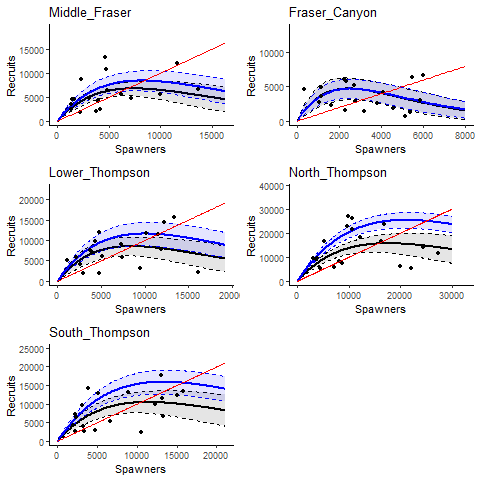
\includegraphics[width=6.67in]{figure/coho-compareSRFits-IM} 

}

\caption{Stock recruit curves fit to spawner and recruitment data using individual models for each CU. Solid black lines shows the MLE fit for the IM model while solid blue lines shows the MLE fit for the IM.HiCap model.  Associated black and blue shaded regions show the 95 percent confidence intervals on respective model fits. The red line show the replacement line.}\label{fig:coho-SR-fit}
\end{figure}

\emph{Model 3: Hierarchical Ricker (HM)}

The hierarchical Ricker model (HM) follows recent stock-recruitment
analyses for Interior Fraser Coho that assume CU-level productivities
are sampled from a common, normal distribution that is shared by all CUs
({[}@korman\_evaluation\_2019{]}, {[}@arbeider\_interior\_2020{]}). The
formulation of the hierarchical Ricker model is the same as that
described above for the individual Ricker model, except we fit it as a
mixed-effect model that treated CU-level \(\alpha_i\) parameters as
random effects:

\begin{equation}
  log(\alpha_i) \sim Normal(\mu_{\alpha},\sigma_{\alpha})
  (\#eq:alpha-HM-dist)
\end{equation}

where, \(\mu_{\alpha}\) is the mean of the normal distribution and
\(\sigma_{\alpha}\) is the standard deviation. In addition to the
likelihood constraints on \(\gamma\) and \(\sigma_{v_i}\) desribed for
the IM, we included the following constraints on \(mu_{\alpha}\) and
\(\sigma_{\alpha}\) to replicate the Bayesian model fitting routine of
@arbeider\_interior\_2020:

\begin{equation}
  log(\mu_{\alpha}) \sim Normal(1,\sqrt{2})
\end{equation}

\begin{equation}
  log(\sigma_{\alpha}) \sim Inverse Gamma (0.1,0.1)
\end{equation}

\emph{Model 4: Hierarchical Ricker with High \(S_Rep\) (HM.HiCap)}

The HM.HiCap model is the same as the IM.HiCap model, but with a
hierarchical structure assumed for CU-level productivities. As with the
HM model (model 3), CU-level productivities are sampled from a common,
normal distribution that is shared by all CUs.

\emph{Calculation of Sgen}

The inclusion of a marine survival co-variate in all four spawner recuit
models means that the realized productivity changes from year to year
with changing marine survival. We incorporated this adjustment into our
calculations of \(S_{gen}\) by first calculating the effective
productivity for each CU as:

\begin{equation}
  log(\alpha'_{i}) = log(\alpha_i) + \gamma log(\overline{m})
   (\#eq:adjProd)
\end{equation}

where, \(\overline{m}\) is the average marine survival rate over the
available time series.

\(S_{MSY}\) was calculated as a function of log(\(\alpha_i'\)) and
\(\beta_i\) using:

\begin{equation}
  S_{MSY,i} = 1 - \frac{W(e^1-\alpha'_i)}{\beta_i} 
   (\#eq:Smsy)
\end{equation}

where, \(W\) represents the Lambert W function (Scheurell 2016).
\(S_{gen}\) was then calculated numerically by solving the following
equation:

\begin{equation}
  S_{MSY} = S_{gen}e^log(\alpha)-\beta_iS_{gen}
  (\#eq:Sgen)
\end{equation}

\textbf{Distribution among subpopulations}

The second type of CU benchmark is based on the distribution of spawning
escapement among subpopulations nested within CUs (Table
@ref(tab:cohoCU2SP)). We have based this benchmark on the short-term
recovery objective identified by the
@ifcrt\_interior\_fraser\_coho\_recovery\_team\_conservation\_2006,
which @arbeider\_interior\_2020 summarized as: \emph{``the 3-year
geometric average, natural-origin escapement in at least half of the
subpopulations within each of the five populations is to exceed 1000
spawning Coho Salmon, excluding hatchery fish spawning in the wild''},
where `populations' is analogous to CUs. We selected the short-term
recovery target to represent a lower CU benchmark in our study because,
as noted by @arbeider\_interior\_2020, the short-term target was
designed as an immediate target when the population was endangered. As
such, it was interpreted as a level expected to prevent extinction or
loss of genetic diversity. The ``half of sub-populations within each
CU'' threshold required 2 out of 3 sub-populations to be above 1000 fish
for the North Thompson and South Thompson CUs, 1 out of 2
sub-populations to be above 1000 fish for the Lower Thompson and Middle
Fraser CUs, and the only sub-population in the Fraser Canyon to be above
1000 fish. This distributional benchmark is specific to the Interior
Fraser Coho SMU. We have retained it as part of this case study to
maintain consistency with previous work.

\hypertarget{lrp-estimation-proportion-of-cus-lower-benchmark}{%
\subsubsection{LRP Estimation: Proportion of CUs \textgreater{} Lower
Benchmark}\label{lrp-estimation-proportion-of-cus-lower-benchmark}}

\textbf{Methods}

We looked at the proportion of CUs that dropped below two types of lower
benchmark to determine in which years between 1998 and 2020 the LRP
would have been breached: (i) Sgen (Figure @ref(fig:coho-CU-timeseries))
and (ii) the proportion of CUs that failed to meet the distributional
target of 1000 fish in half of subpopulations
@ref(fig:coho-Subpop-EscpSeries)) . Status was assessed as being below
the LRP in years in which one or more CUs was below their CU-level
benchmark. Estimates of Sgen were based on all data available up to
2020, so our evaluation is not a true retrospective analysis in which
only the data available up to each year in a time series are used to
estimate status.

\begin{figure}

{\centering 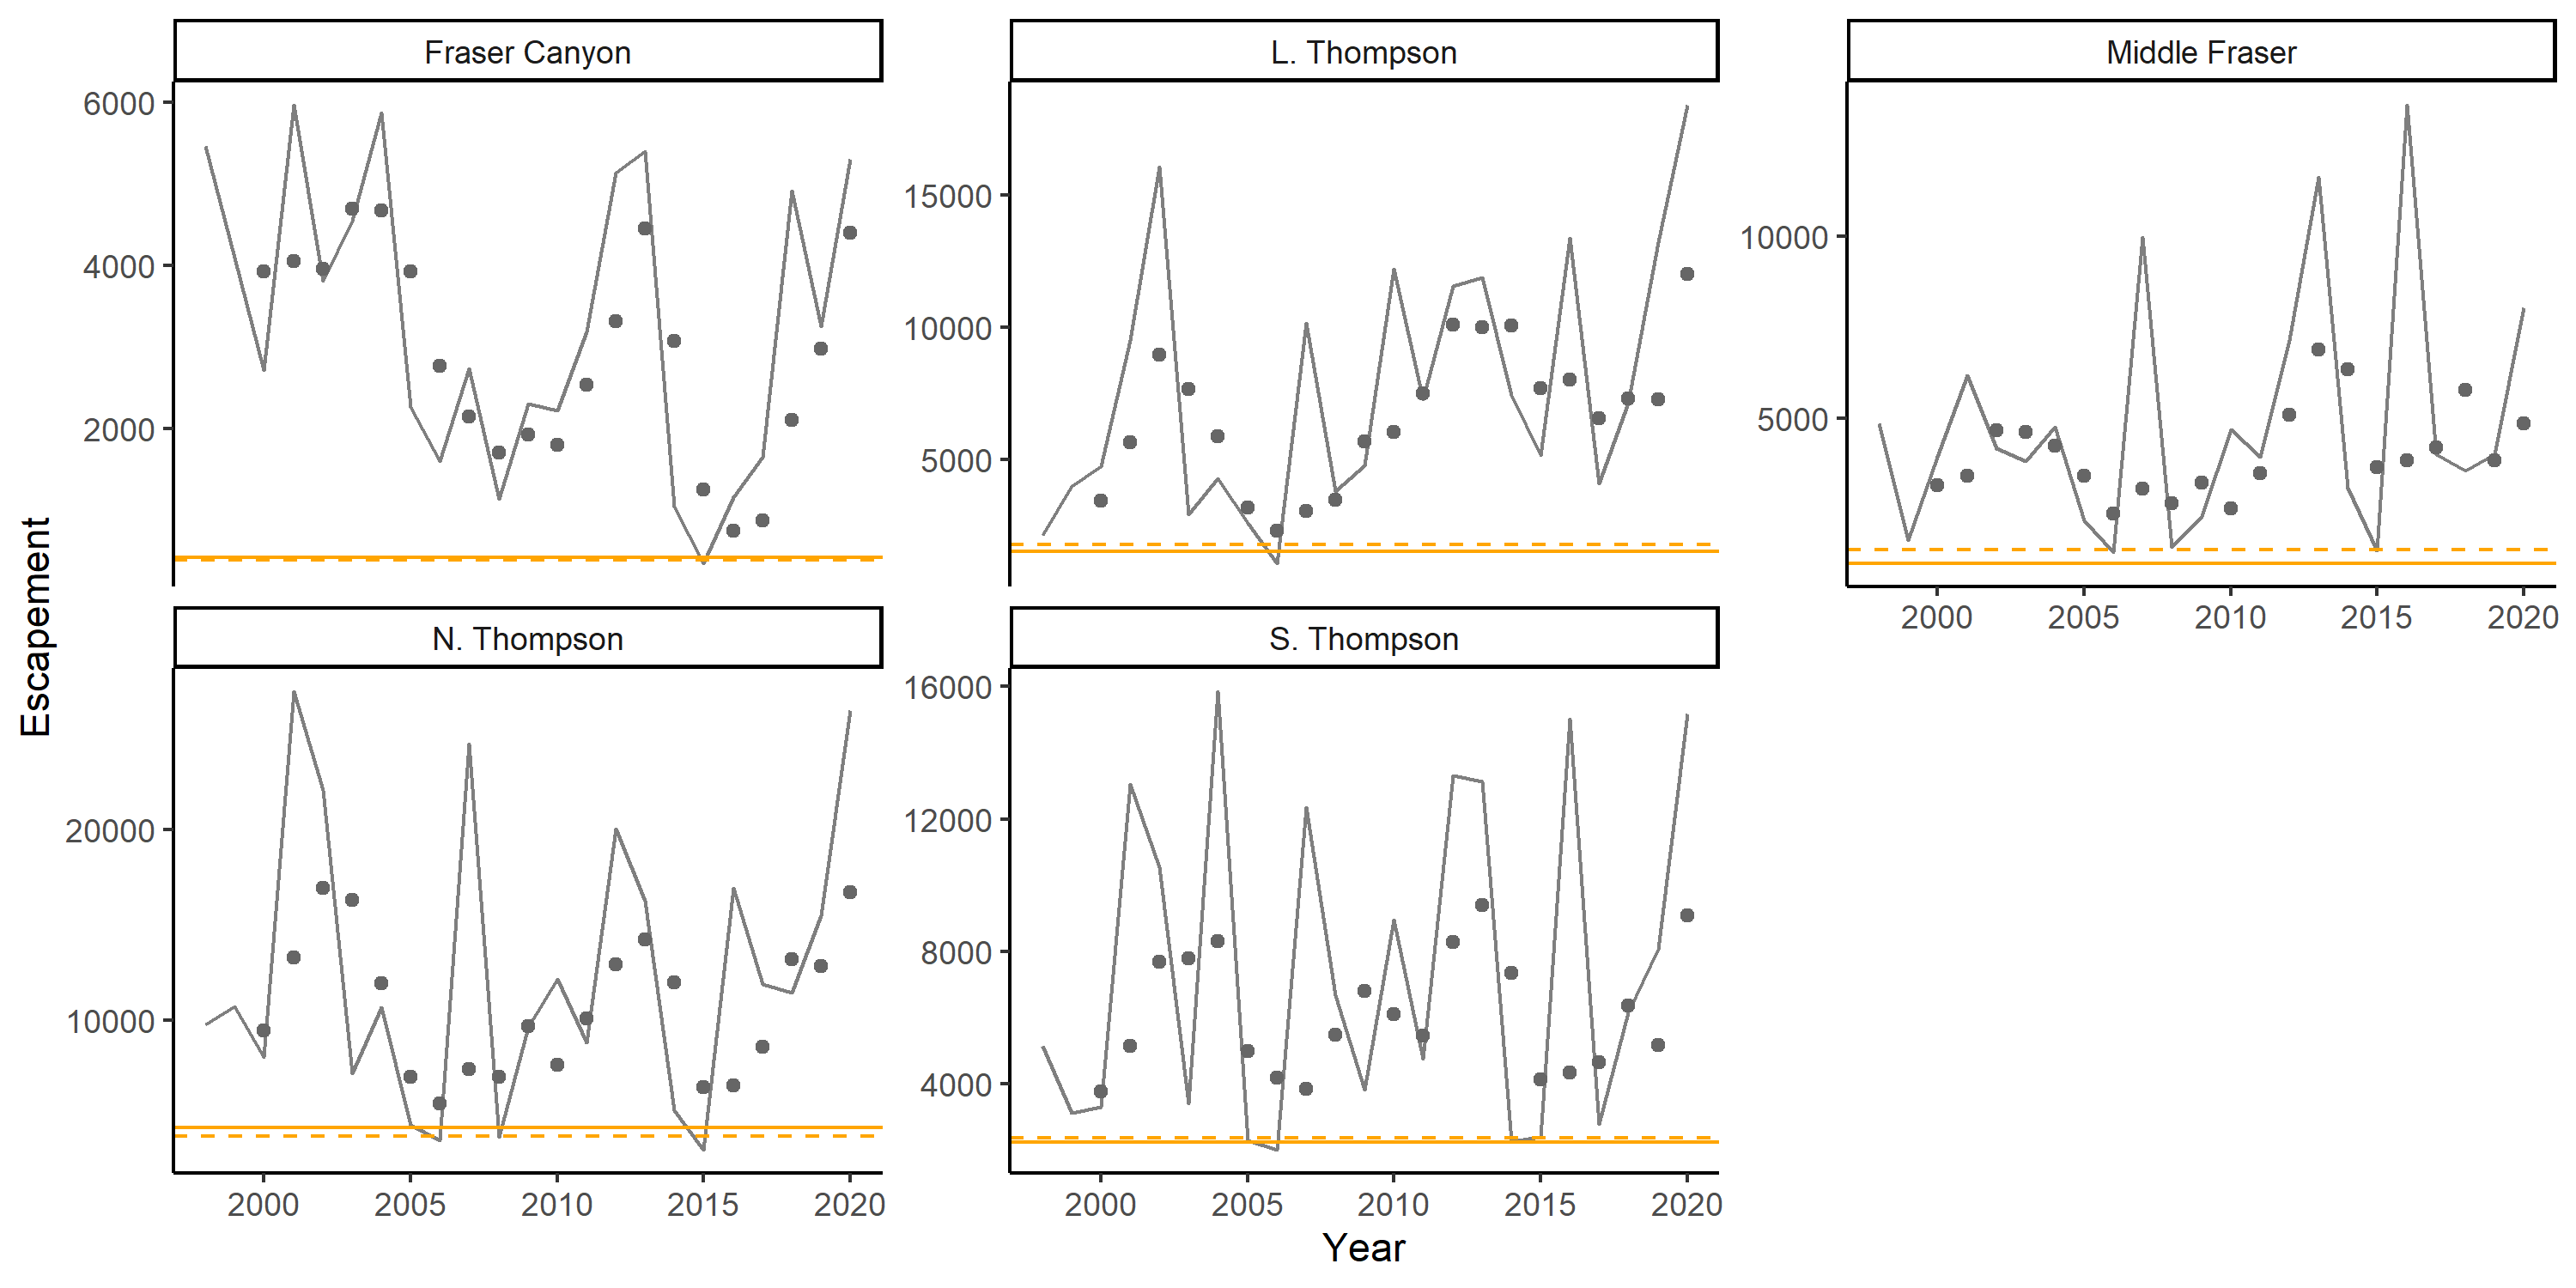
\includegraphics[width=41.67in]{figure/coho-CU-EscpSeries-wStatus} 

}

\caption{Escapement time series for five Interior Fraser Coho CUs shown as annual escapements (lines) and 3-year geometric mean escapements (dots). Solid orange lines show estimates of Sgen from the IM model, while dashed orange lines show estimates of Sgen from the IM.HiCap model.}\label{fig:coho-CU-timeseries}
\end{figure}

\begin{figure}

{\centering 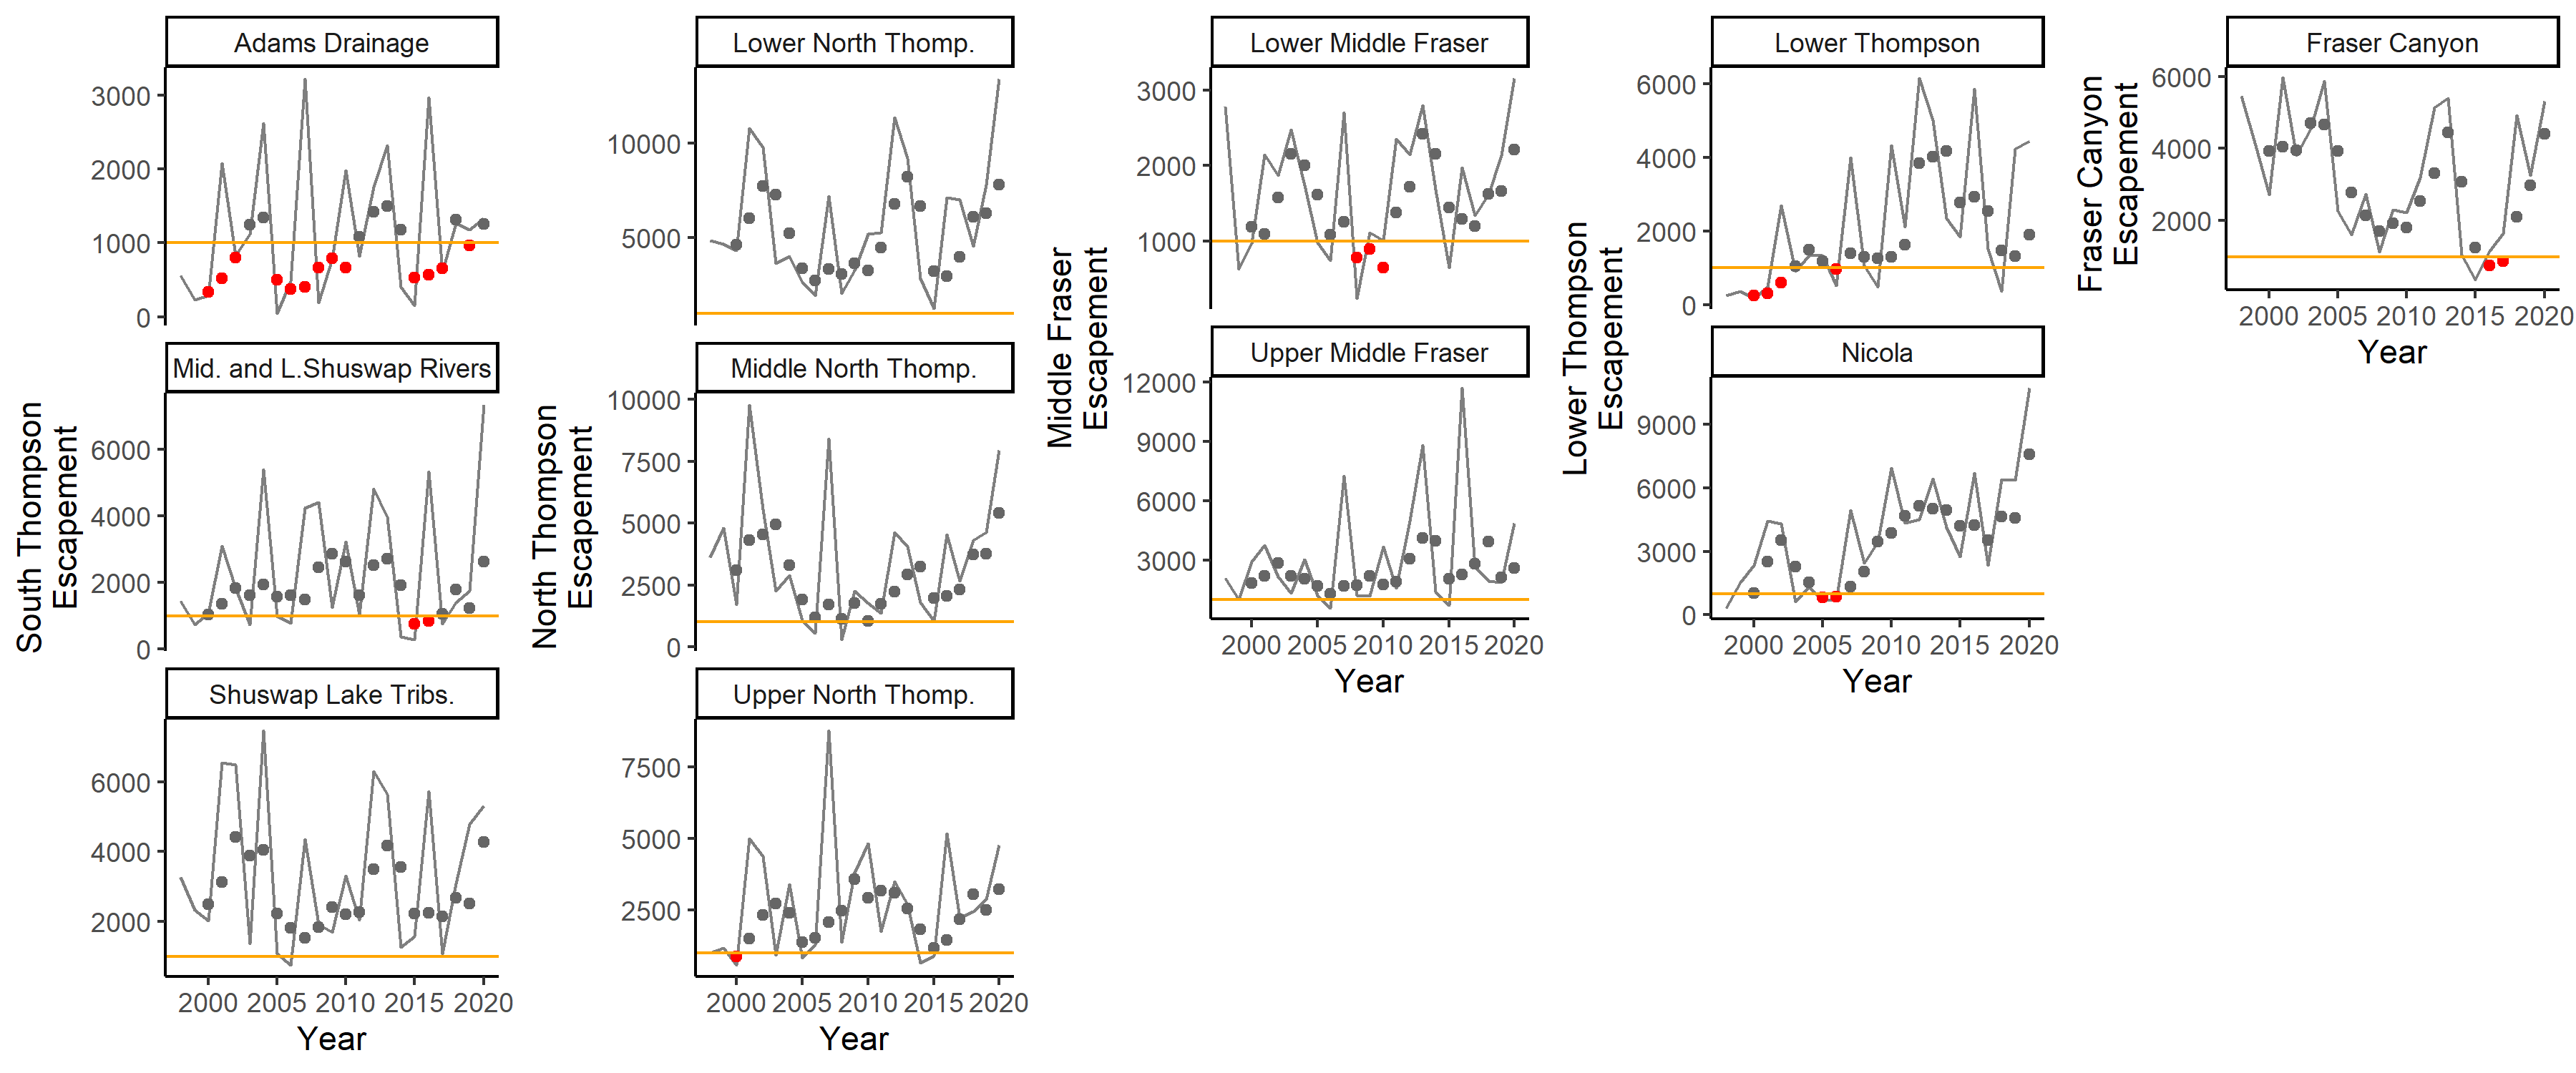
\includegraphics[width=41.67in]{figure/coho-Subpop-EscpSeries-wStatus} 

}

\caption{Escapement time series for 11 subpopulations of Interior Fraser Coho shown as annual escapements (lines) and 3-year geometric mean escapements (dots). Gray dots shows years in which the 3-year geometric mean escapement was above the 1000 fish threshold used to assess distributional status, while red dots show years in which the 1000 fish threshold was not met.  CUs to which each subpopulation belong to are shown in Table --}\label{fig:coho-Subpop-timeseries}
\end{figure}

\linebreak

\textbf{Results}

Estimates of Sgen based on the IM.cap spawner recruit model were higher
than those based on the IM model for three of the five CUs (Middle
Fraser, Lower Thompson, and South Thompson) and were approximately equal
for another CU (Fraser Canyon; Figure @ref(fig:coho-CU-timeseries). As a
result, we would expect the use of the IM.cap model to trigger an LRP
breach at lower CU level abundances in most cases. However, generational
average abundances remained high enough between 2000 and 2020 to avoid
this happening. For all five CUs, the generational (3-year) geometric
average escapement between 2000 and 2020 remained above the 2020
estimate of Sgen (\(Sgen_{2020}\)), regardless of which stock recruit
model was used to estimate Sgen (Figure @ref(fig:coho-CU-timeseries)).
Because the proportion of CUs above Sgen was always 100\%, there were no
years in which a trigger-based LRP that required 100\% of CUs to be
above Sgen would have been breached.

In contrast, the SMU-level LRP was breached in 4 of the 21 years between
2000 and 2020 years when the distributional CU benchmark was used to
characterize CU-level status instead of Sgen for the proportion-based
LRP. Eight of the 11 sub-populations had generational average escapement
drop below the 1000 spawner threshold in one or more years (Figure
@ref(fig:coho-Subpop-timeseries)). Sub-populations tended to differ in
which years they dropped below the 1000 spawner threshold, which meant
that the distributional benchmark at least half of the subpopulations
within each CU with greater than 1000 fish was more often met than not.
All 11 subpopulations had generational average spawning abundances above
1000 spawners in 2020, indicating that the stock would be well above a
proportional LRP based on the distributional benchmark (Figure
@ref(fig:coho-Subpop-timeseries)).

\hypertarget{lrp-estimation-aggregate-abundance-empirical-lrps}{%
\subsubsection{LRP Estimation: Aggregate Abundance Empirical
LRPs}\label{lrp-estimation-aggregate-abundance-empirical-lrps}}

\textbf{Methods}

We evaluated aggregate abundance-based LRPs derived using logistic
regressions for both types of Interior Fraser Coho benchmarks: Sgen and
the distributional target of 1000 fish in half of sub-populations. See
Section @ref(logisticMethods) for an overview of the approach used to
calculate aggregate abundance-based LRPs using logistic regression.

When estimating logistic regression LRPs using Sgen, we used an
integrated modelling approach in which CU-level Sgen and the SMU-level
LRP were simultaneously estimated. The integrated Sgen-LRP models had
two components:

\begin{enumerate}
\def\labelenumi{(\roman{enumi})}
\item
  Stock-recruit models fit to each of the 5 CUs to estimate CU-level
  Sgen (Equation @ref(eq:rickerSurv-IM) and Equations @ref(eq:adjProd) -
  @ref(eq:Sgen))
\item
  A logistic regression model fit to aggregated data to estimate the LRP
  as the aggregate abundance that has historically been associated with
  a specified probability of all CUs being above Sgen (Equations
  @ref(eq:logistic) - @ref(eq:logisticLRP))
\end{enumerate}

\textbf{\emph{Retrospective Analysis}}

We used a retrospective analysis to examine the effect of time series
length on aggregate abundance-based LRP estimates when using the
logistic regression approach. Retrospective analyses were restricted to
the most recent x years (2015-2020) because logistic model fits prior to
xxxx were unable to converge on an LRP estimate. For each year between
xxxx and xxxx, we used data only available up to that year to calculate
LRPs and associated confidence intervals.

\textbf{\emph{Effect of Missing CUs}}

To examine the effect of missing CUs on LRP estimates, we calculated
LRPs using data from only a subset of the five Interior Fraser Coho CUs.
We limited our analysis to missing data from either one or two CUs so
that we had at least three CUs of available data when calculating the
proportion of CUs above their benchmarks. For each missing data case, we
calculated SMU status as

\begin{equation}
  Status_t = \frac{\sum_{i}^{nCUs} S_{i,t}}{LRP'_t}
   (\#eq:status)
\end{equation}

where \(nCUs\) is the number of CUs being used (3 or 4) and \(LRP'_t\)
is the LRP calculated in year \(t\) using only data from \(nCUs\).
SMU-level status in a given year was calculated for all possible
combinations of CUs available (5 combinations when nCUs = 4 and 10
combinations when nCUs = 3) to allow examination of the stability of
status estimates among available combinations. Estimates of SMU status
relative to LRPs were used to compare among missing CU scenarios instead
of absolute LRP estimates because absolute LRP estimates vary with the
number (and combination) of CUs used.

\textbf{Results}

\textbf{\emph{Logistic LRP Estimates in 2020}}

Logistic regression model fits in 2020 to CU-level status predictions
from Sgen:IM and Sgen:IM.Cap models are shown in Figures
@ref(fig:coho-IM-logisticFit2020) and
@ref(fig:coho-IMCap-logisticFit2020), respectively, while the logistic
regression model fit to status estimates based on the IFCRT short-term
distributional target is shown in Figure
@ref(fig:coho-Distr-logisticFit2020).

To Add: Appendix: Maximum posterior density estimates (± standard error)
obtained from fitting the `Individual Ricker' (IM) version of the
Integrated Sgen-LRP model to Interior Fraser Coho data.

To Add: Appendix: Maximum posterior density estimates (± standard error)
obtained from fitting the `Individual Ricker with cap' (IM.cap) version
of the Integrated Sgen-LRP model to Interior Fraser Coho data.

All three estimation methods for IFC logistic regression-based LRPs were
able to converge on a solution. Resulting LRPs for different p\^{}*
thresholds are shown on the regression curves, as well as in Table
@ref(tab:logisticLRPs2020). There was however considerable uncertainty
around predicted curves as seen in the large areas of gray shading in
Figures @ref(fig:coho-IM-logisticFit2020) -
@ref(fig:coho-Distr-logisticFit2020).

\begin{figure}

{\centering 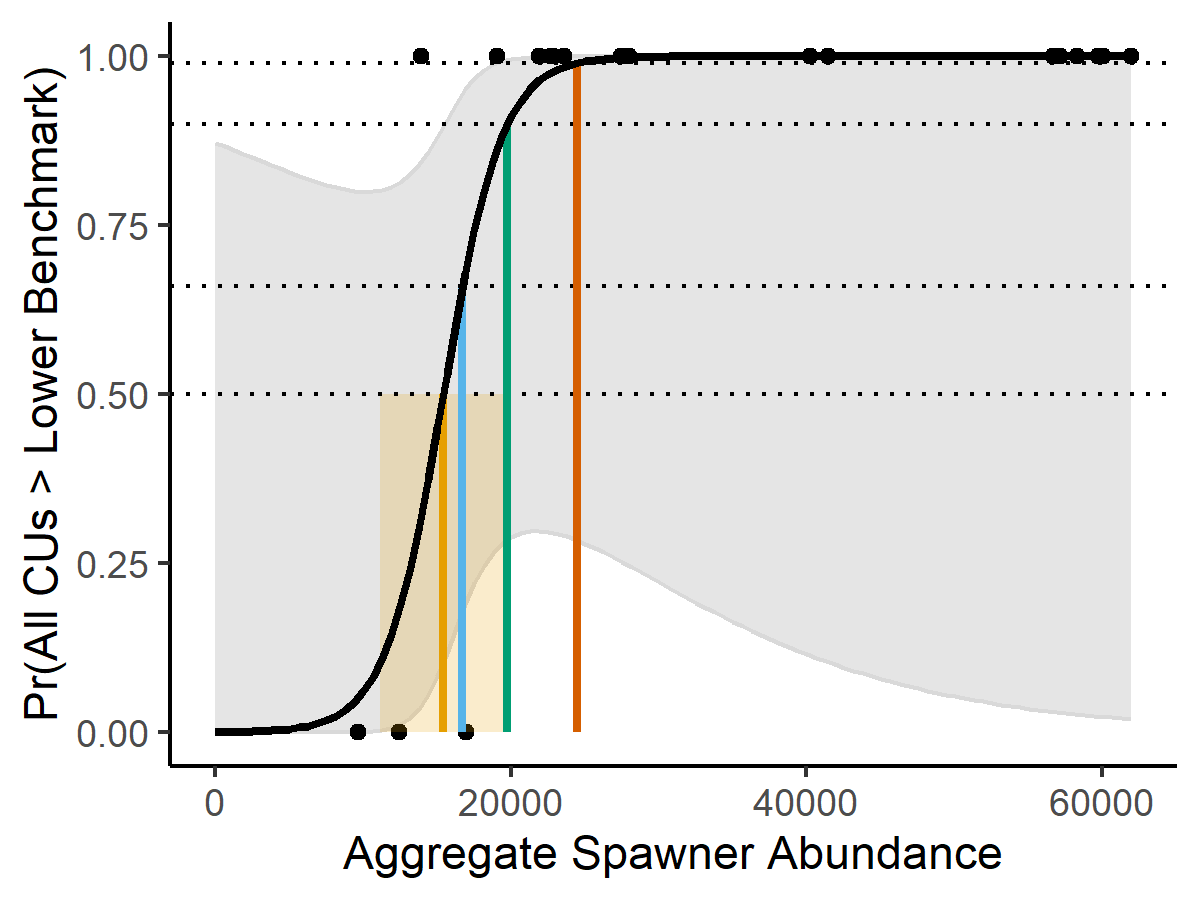
\includegraphics[width=0.5\linewidth]{figure/coho-IM2020-LogisticLRP} 

}

\caption{Logistic regression fit to CU-level status predictions from the Integrated Sgen-LRP model (1998 - 2020), where the logistic model is used to predict the probability that all CUs are above Sgen when Sgen is estimated using the IM spawner recruit model. The yellow vertical line shows the aggregate abundance-based LRP estimate based on the requirement of a 50\% probability of all CUs being above Sgen, while the yellow shaded region shows the associated 95\% confidence interval around the LRP. LRPs (MLE estimates only; no confidence intervals) for three alternative probability thresholds, 66\%, 90\%, and 99\%, are shown in blue, green, and orange, respectively.}\label{fig:coho-IM-logisticFit2020}
\end{figure}

When the Sgen:IM integrated LRP model was used, aggregate
abundance-based LRPs ranged from 15,395 to 24,331 spawners, depending on
whether the required probability of all CUs being above Sgen was
moderate (50\%) or very likely (99\%) (Table
@ref(tab:logisticLRPs2020)). LRPs increased across all probability
levels when the carrying capacity was assumed higher under the
Sgen:IMCap model (Table @ref(tab:logisticLRPs2020)). The higher Sgen
values for most CUs under this alternative model formulation resulted in
more historical years in which \textless{} 100\% of CUs were above Sgen.
Several years with aggregate abundances between 19,000 - 30,000 spawners
that had met the threshold of all CUs \textgreater{} Sgen using the IM
model no longer met this threshold, resulting in a shift of the fit
curve to the right and higher LRP estimates. LRPs based on the IMCap
model ranged from 25,677 to 40,784 spawners, depending on whether the
required probability of all CUs being above Sgen was moderate (50\%) or
very likely (99\%).

\begin{figure}

{\centering 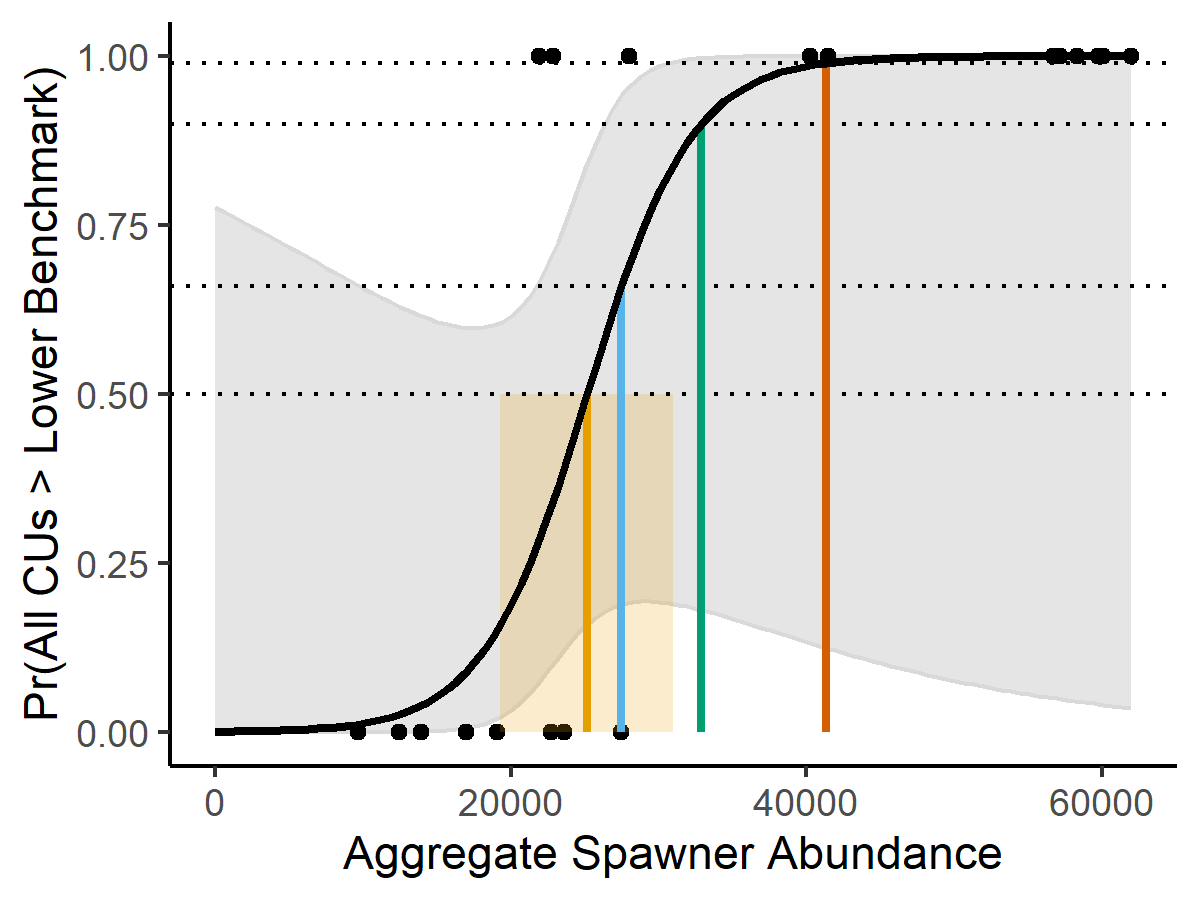
\includegraphics[width=0.5\linewidth]{figure/coho-IMCap2020-LogisticLRP} 

}

\caption{Logistic regression fit to CU-level status predictions from the Integrated Sgen-LRP model (1998 - 2020), where the logistic model is used to predict the probability that all CUs are above Sgen when Sgen is estimated using the IM.HiCap spawner recruit model. See Figure x caption for additional details.}\label{fig:coho-IMCap-logisticFit2020}
\end{figure}

When CU status was based on the IFCRT short-term distributional target,
the fit logistic curve was more gradual than the two Sgen models due to
a greater overlap in `successful' (all CUs \textgreater{} distributional
target) and `unsuccessful' (\textless100\% of CUs above distributional
target) years at low to moderate aggregate abundances. In 3 of the 6
years with aggregate abundances below 20,000 spawners, the
distributional target was not met for all CUs (Figure
@ref(fig:coho-Distr-logisticFit2020)). As a result, LRPs based on the
IFCRT short-term distributional target were more uncertain than those
based on Sgen. LRPs based on this model also became increasingly large
at high probability thresholds (Table @ref(tab:logisticLRPs2020). The
LRP based on a 50\% probability that all CUs would be above their
distributional targets was 17,515 spawners (95\% CI = 9,695 - 25,336)
while the LRP based on a 99\% probability was 44,403 spawners (95\% CI =
15,102 - 73,703).

\begin{figure}

{\centering 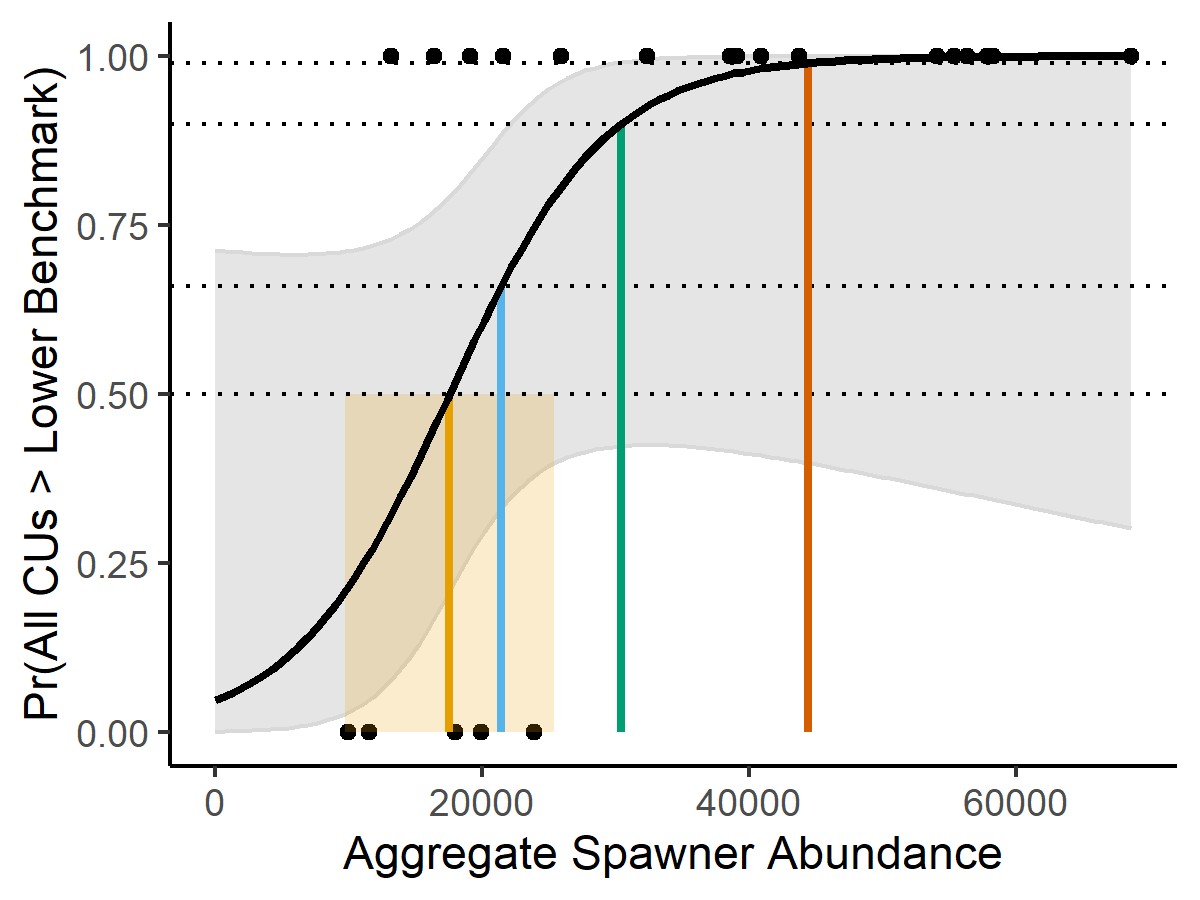
\includegraphics[width=0.5\linewidth]{figure/coho-ThreshAb2020-LogisticLRP} 

}

\caption{Logistic regression fit to observed escapement data (1998 - 2020) to predict the probability that all CUs are above the IFCRT short-term distributional target. See Figure x caption for additional details.}\label{fig:coho-Distr-logisticFit2020}
\end{figure}

\begin{longtable}[]{@{}llll@{}}
\caption{(\#tab:logisticLRPs2020) Aggregate abundance based LRPs (with
95\% confidence intervals) from logistic regressions applied to three
alternative CU lower benchmarks (Sgen:IM, Sgen:IM.HiCap, and
Distributional). For each probability level, the LRP estimate represents
that probability that all CUs will be above their lower
benchmark.}\tabularnewline
\toprule
\begin{minipage}[b]{0.17\columnwidth}\raggedright
Probability\strut
\end{minipage} & \begin{minipage}[b]{0.22\columnwidth}\raggedright
Sgen: IM\strut
\end{minipage} & \begin{minipage}[b]{0.22\columnwidth}\raggedright
Sgen:IM.HiCap\strut
\end{minipage} & \begin{minipage}[b]{0.22\columnwidth}\raggedright
Distributional\strut
\end{minipage}\tabularnewline
\midrule
\endfirsthead
\toprule
\begin{minipage}[b]{0.17\columnwidth}\raggedright
Probability\strut
\end{minipage} & \begin{minipage}[b]{0.22\columnwidth}\raggedright
Sgen: IM\strut
\end{minipage} & \begin{minipage}[b]{0.22\columnwidth}\raggedright
Sgen:IM.HiCap\strut
\end{minipage} & \begin{minipage}[b]{0.22\columnwidth}\raggedright
Distributional\strut
\end{minipage}\tabularnewline
\midrule
\endhead
\begin{minipage}[t]{0.17\columnwidth}\raggedright
50\%\strut
\end{minipage} & \begin{minipage}[t]{0.22\columnwidth}\raggedright
15,395 (11,187-19,603)\strut
\end{minipage} & \begin{minipage}[t]{0.22\columnwidth}\raggedright
25,677 (20,683-30,672)\strut
\end{minipage} & \begin{minipage}[t]{0.22\columnwidth}\raggedright
17,515 (9,695-25,336)\strut
\end{minipage}\tabularnewline
\begin{minipage}[t]{0.17\columnwidth}\raggedright
66\%\strut
\end{minipage} & \begin{minipage}[t]{0.22\columnwidth}\raggedright
16,685 (12,454-20,916)\strut
\end{minipage} & \begin{minipage}[t]{0.22\columnwidth}\raggedright
27,858 (21,674-34,042)\strut
\end{minipage} & \begin{minipage}[t]{0.22\columnwidth}\raggedright
21,396 (13,418-29,375)\strut
\end{minipage}\tabularnewline
\begin{minipage}[t]{0.17\columnwidth}\raggedright
90\%\strut
\end{minipage} & \begin{minipage}[t]{0.22\columnwidth}\raggedright
19,668 (13,752-25,584)\strut
\end{minipage} & \begin{minipage}[t]{0.22\columnwidth}\raggedright
32,901 (22,257-43,544)\strut
\end{minipage} & \begin{minipage}[t]{0.22\columnwidth}\raggedright
30,372 (15,711-45,033)\strut
\end{minipage}\tabularnewline
\begin{minipage}[t]{0.17\columnwidth}\raggedright
99\%\strut
\end{minipage} & \begin{minipage}[t]{0.22\columnwidth}\raggedright
24,331 (13,924-34,738)\strut
\end{minipage} & \begin{minipage}[t]{0.22\columnwidth}\raggedright
40,784 (21,957-59,610)\strut
\end{minipage} & \begin{minipage}[t]{0.22\columnwidth}\raggedright
44,403 (15,102-73,703)\strut
\end{minipage}\tabularnewline
\bottomrule
\end{longtable}

\textbf{\emph{Logistic Regression Diagnostics}}

Logistic regression diagnostics for all three models indicated some
problems with model fits (Table @ref(tab:logisticDiagIFC2020)).
Assumptions of linearity, a lack of influential outliers, and
independence among observation were met for all models. The assumption
of linearity was demonstrated based on non-significant interaction terms
from the Box-Tidwell test. An examination of deviance residuals did not
show any influential outliers, and the absolute magnitude of lag-1 AR
correction in deviance residuals was always \(\leq\) 0.20 indicating
that annual observations were independent of each other. However,
diagnostic tests on model fits to data yielded mixed results. The Wald
Test showed that logistic model coefficients were either marginally
significant (0.05 \textless{} p \textless0.10) or just above the
marginally significant threshold for all three models. Quasi-\(R^2\)
statistics indicated a moderately strong relationship between aggregate
abundance and the probability of all CUs being above their lower
benchmarks. Quasi-\(R^2\) values were 0.68 and 0.63 for the two Sgen
models, and 0.41 for the model based on the IRCRT distributional target.
However despite moderate quasi-\(R^2\) values, goodness of fit
statistics indicated a significant lack of fit based on p-values less
than 0.001.

Minimum sample size requirements were not met for any models, meaning
that available data sets were not large enough to support valid
conclusions from fitted models. Based on a minimum requirement of 10
data points for the least frequent outcome, the minimum sample size for
the Sgen:IM model was 77 years. This requirement was substantially
higher than the 23 years of available data. Minimum sample sizes for the
Sgen:IMCap and Distributional model were smaller. The requirement for
the Sgen:IMCap model was 26 years, which was just above the available 23
years. The requirement for the model based on the IFCRT Distributional
target was 42 years.

Finally, `hit ratios' representing classification accuracy as the ratio
of successful classifications to total number of data points were
relatively high at low probability thresholds, indicating good accuracy.
This results was especially for the Sgen:IM model which had a hit ratio
0f 0.91 at probability thresholds of 50\%, 66\%, and 90\%.
Classification accuracy was lowest for all models at the 99\%
probability threshold.

\begin{longtable}[]{@{}llll@{}}
\caption{(\#tab:logisticDiagIFC2020) Model diagnostic statistics from
logistic regressions applied to three alternative CU lower benchmarks
(Sgen:IM, Sgen:IM.HiCap, and Distributional). A description of
diagnostic tests is provided in Section \ldots{}}\tabularnewline
\toprule
\begin{minipage}[b]{0.30\columnwidth}\raggedright
Diagnostic Test\strut
\end{minipage} & \begin{minipage}[b]{0.17\columnwidth}\raggedright
Sgen: IM\strut
\end{minipage} & \begin{minipage}[b]{0.21\columnwidth}\raggedright
Sgen:IM.HiCap\strut
\end{minipage} & \begin{minipage}[b]{0.21\columnwidth}\raggedright
Distributional\strut
\end{minipage}\tabularnewline
\midrule
\endfirsthead
\toprule
\begin{minipage}[b]{0.30\columnwidth}\raggedright
Diagnostic Test\strut
\end{minipage} & \begin{minipage}[b]{0.17\columnwidth}\raggedright
Sgen: IM\strut
\end{minipage} & \begin{minipage}[b]{0.21\columnwidth}\raggedright
Sgen:IM.HiCap\strut
\end{minipage} & \begin{minipage}[b]{0.21\columnwidth}\raggedright
Distributional\strut
\end{minipage}\tabularnewline
\midrule
\endhead
\begin{minipage}[t]{0.30\columnwidth}\raggedright
Box-Tidwell p-value\strut
\end{minipage} & \begin{minipage}[t]{0.17\columnwidth}\raggedright
0.81\strut
\end{minipage} & \begin{minipage}[t]{0.21\columnwidth}\raggedright
1.0\strut
\end{minipage} & \begin{minipage}[t]{0.21\columnwidth}\raggedright
0.79\strut
\end{minipage}\tabularnewline
\begin{minipage}[t]{0.30\columnwidth}\raggedright
Max. deviance residual\strut
\end{minipage} & \begin{minipage}[t]{0.17\columnwidth}\raggedright
1.52\strut
\end{minipage} & \begin{minipage}[t]{0.21\columnwidth}\raggedright
1.68\strut
\end{minipage} & \begin{minipage}[t]{0.21\columnwidth}\raggedright
1.66\strut
\end{minipage}\tabularnewline
\begin{minipage}[t]{0.30\columnwidth}\raggedright
AR-1\strut
\end{minipage} & \begin{minipage}[t]{0.17\columnwidth}\raggedright
-0.20\strut
\end{minipage} & \begin{minipage}[t]{0.21\columnwidth}\raggedright
0.16\strut
\end{minipage} & \begin{minipage}[t]{0.21\columnwidth}\raggedright
0.05\strut
\end{minipage}\tabularnewline
\begin{minipage}[t]{0.30\columnwidth}\raggedright
Min. sample size\strut
\end{minipage} & \begin{minipage}[t]{0.17\columnwidth}\raggedright
77\^{}*\strut
\end{minipage} & \begin{minipage}[t]{0.21\columnwidth}\raggedright
26\^{}*\strut
\end{minipage} & \begin{minipage}[t]{0.21\columnwidth}\raggedright
42\^{}*\strut
\end{minipage}\tabularnewline
\begin{minipage}[t]{0.30\columnwidth}\raggedright
Wald p-values (\(B_0\), \(B_1\))\strut
\end{minipage} & \begin{minipage}[t]{0.17\columnwidth}\raggedright
\(B_0\): 0.11 + \(B_1\): 0.09 +\strut
\end{minipage} & \begin{minipage}[t]{0.21\columnwidth}\raggedright
\(B_0\): 0.06 + \(B_1\): 0.08 +\strut
\end{minipage} & \begin{minipage}[t]{0.21\columnwidth}\raggedright
\(B_0\): 0.13 \(B_0\): 0.09\strut
\end{minipage}\tabularnewline
\begin{minipage}[t]{0.30\columnwidth}\raggedright
Goodness-of-fit p-value\strut
\end{minipage} & \begin{minipage}[t]{0.17\columnwidth}\raggedright
\textless0.01\strut
\end{minipage} & \begin{minipage}[t]{0.21\columnwidth}\raggedright
\textless0.01\strut
\end{minipage} & \begin{minipage}[t]{0.21\columnwidth}\raggedright
\textless0.01\strut
\end{minipage}\tabularnewline
\begin{minipage}[t]{0.30\columnwidth}\raggedright
Quasi-\(R^2\)\strut
\end{minipage} & \begin{minipage}[t]{0.17\columnwidth}\raggedright
0.68\strut
\end{minipage} & \begin{minipage}[t]{0.21\columnwidth}\raggedright
0.63\strut
\end{minipage} & \begin{minipage}[t]{0.21\columnwidth}\raggedright
0.41\strut
\end{minipage}\tabularnewline
\begin{minipage}[t]{0.30\columnwidth}\raggedright
Hit Ratio (p*= 50\%, 60\%, 90\%, 99\%)\strut
\end{minipage} & \begin{minipage}[t]{0.17\columnwidth}\raggedright
0.91, 0.91 0.91, 0.74\strut
\end{minipage} & \begin{minipage}[t]{0.21\columnwidth}\raggedright
0.87, 0.91, 0.87, 0.78\strut
\end{minipage} & \begin{minipage}[t]{0.21\columnwidth}\raggedright
0.76, 0.81, 0.76, 0.52\strut
\end{minipage}\tabularnewline
\bottomrule
\end{longtable}

Despite some of the poor model fit diagnostics for logistic regressions
fit to IFC data, we decided to proceed with retrospective analyses and
an examination of the effect of missing CUs in order to examine how
sensitive LRPs based on these model fits were to variations in the level
of available data.

\textbf{\emph{Retrospective Analysis}}

\begin{figure}

{\centering 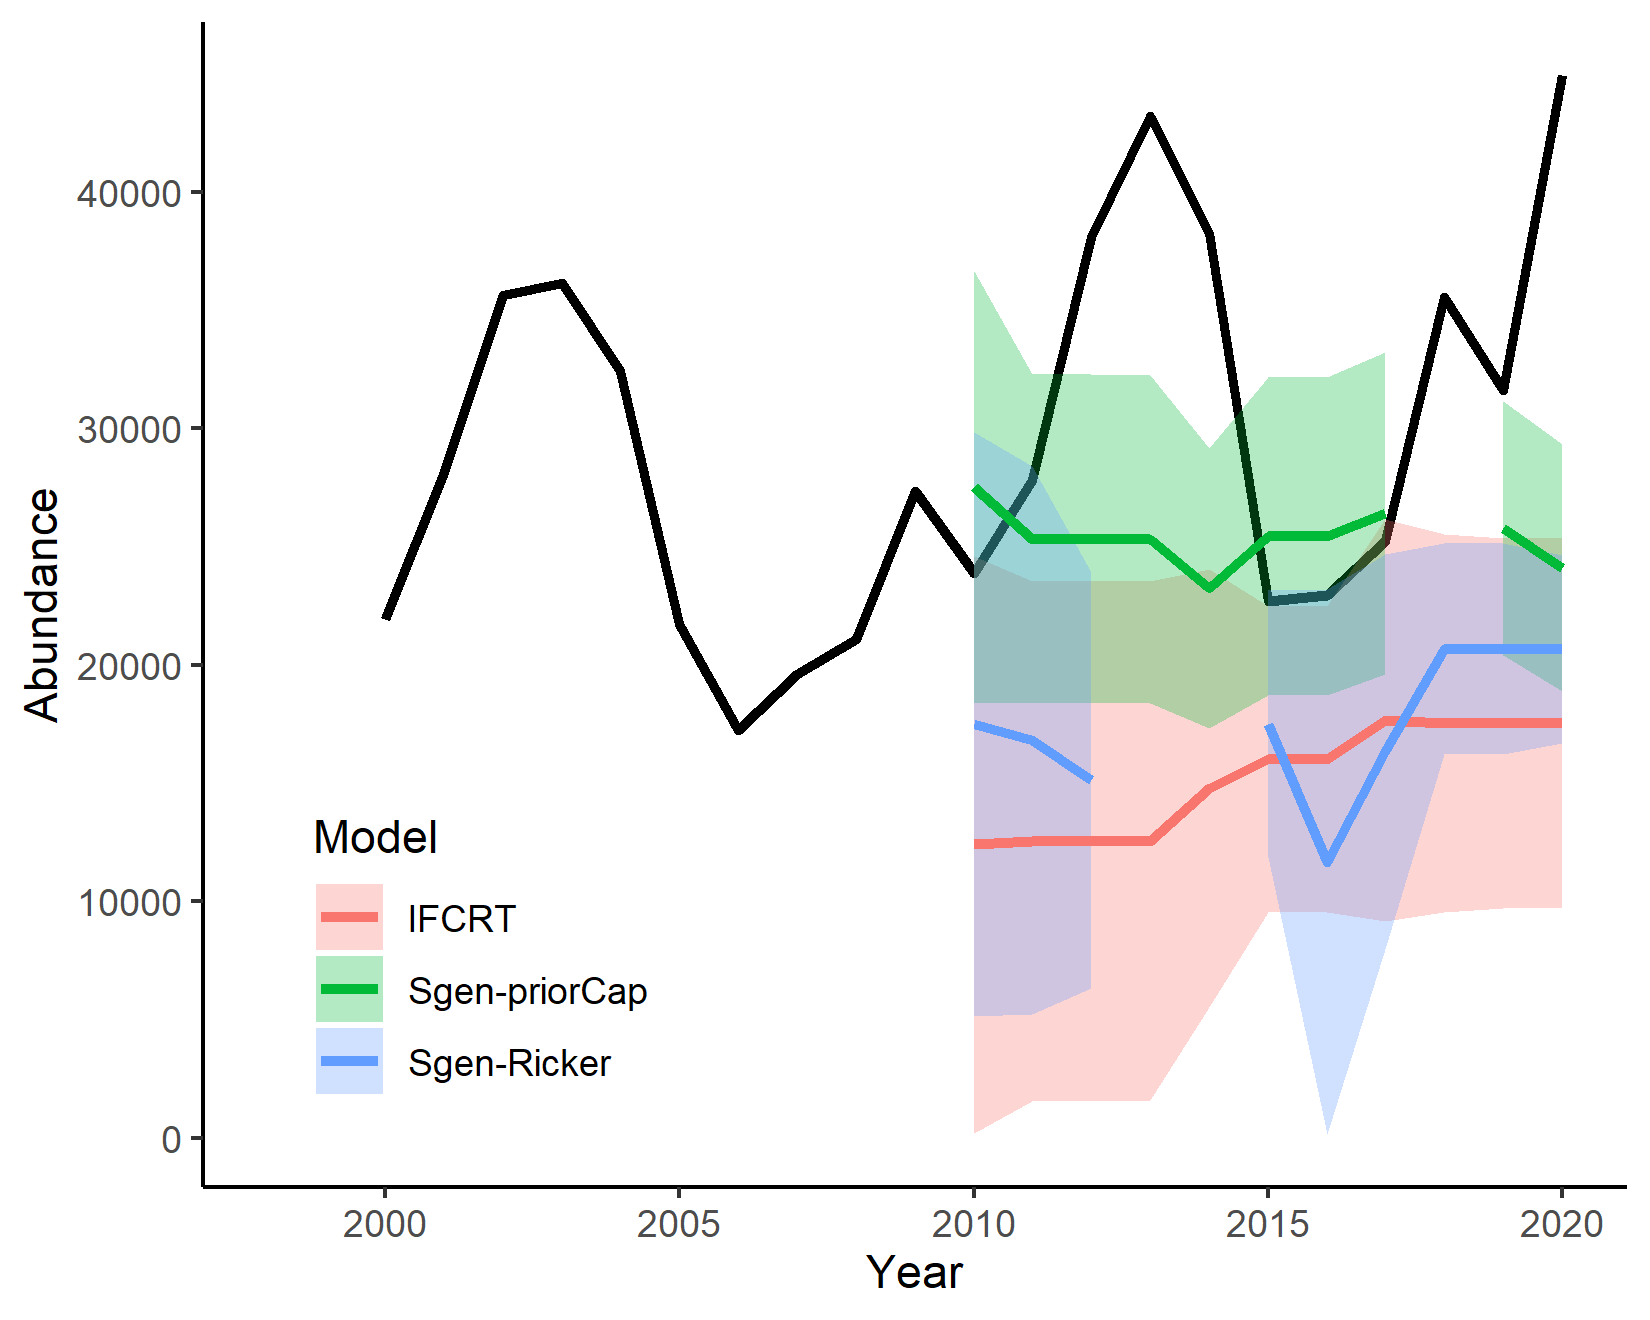
\includegraphics[width=0.5\linewidth]{figure/coho_LRP_compareRetro} 

}

\caption{Three-year geometric mean of aggregate spawning abundance for the Interior Fraser Coho SMU (black line) and associated time series of retrospective LRPs from logistic regression-based estimation methods. LRPs are based on a 50\% probability that all CUs will be above their lower benchmarks. Annual LRP estimates are shown as maximum likelihood values (coloured lines) and associated 95\% confidence intervals (shaded areas).}\label{fig:coho-retroLRPs}
\end{figure}

\textbf{\emph{Effect of Missing CUs}}

\hypertarget{lrp-estimation-aggregate-abundance-projection-based-lrps}{%
\subsubsection{LRP Estimation: Aggregate Abundance Projection-Based
LRPs}\label{lrp-estimation-aggregate-abundance-projection-based-lrps}}

\textbf{Methods}

IM model

IM cap model

Model averaging

\textbf{Results}

\hypertarget{historical-evaluation-of-status-across-lrp-methods}{%
\subsubsection{HISTORICAL EVALUATION OF STATUS ACROSS LRP
METHODS}\label{historical-evaluation-of-status-across-lrp-methods}}

Table: Comparison of all logistic LRP estimates in 2020

\end{document}
